\documentclass{beamer}

\usepackage[utf8]{inputenc}
\usepackage[T1]{fontenc}
\usepackage[english]{babel}
\usepackage{lmodern}
\usepackage{color}
\usepackage{fix-cm}
\usepackage{textpos}
\usepackage{eurosym}
\usepackage{multirow}
\usepackage{perpage}
\usepackage{eso-pic}
\usepackage{times}
\usepackage{tikz}
\usetikzlibrary{matrix}

\usepackage{tikz}
\usepackage{varwidth}
\usetikzlibrary{decorations.text}
\definecolor{dkgreen}{rgb}{0,0.6,0}
\definecolor{gray}{rgb}{0.5,0.5,0.5}
\definecolor{mauve}{rgb}{0.58,0,0.82}
\usepackage{amsmath}
\usetikzlibrary{arrows}




% Redéfinis les marges des tableaux
\let\oldtabular=\tabular
\def\tabular{\small\oldtabular}
\renewcommand{\arraystretch}{1.5}

\colorlet{helpful}{lime!40}
\colorlet{harmful}{red!30}
\colorlet{internal}{yellow!20}
\colorlet{external}{cyan!30}
\colorlet{S}{helpful!50!internal}
\colorlet{W}{harmful!50!internal}
\colorlet{O}{helpful!50!external}
\colorlet{T}{harmful!50!external}

\newcommand{\texta}{Positif\par}
\newcommand{\textb}{Négatif\par}
\newcommand{\textcn}{Interne\par}
\newcommand{\textdn}{Externe\par}

\newcommand{\back}[1]{\fontsize{80}{70}\selectfont #1}
%%%

\graphicspath{{images/}}

\newcommand{\placetextbox}[3]{% \placetextbox{<horizontal pos>}{<vertical pos>}{<stuff>}
	\setbox0=\hbox{#3}% Put <stuff> in a box
	\AddToShipoutPictureFG*{% Add <stuff> to current page foreground
		\put(\LenToUnit{#1\paperwidth},\LenToUnit{#2\paperheight}){\vtop{{\null}\makebox[0pt][c]{#3}}}%
	}%
}%

% Redéfinis les marges des tableaux
\let\oldtabular=\tabular
\def\tabular{\small\oldtabular}
\renewcommand{\arraystretch}{1.5}

\usetheme{Warsaw}
\usecolortheme{orchid}
\graphicspath{{graphics/}}

% Permet de réinitialiser les footnote à chaque frame. Nécéssite 2 compilations.
\MakePerPage{footnote}

\setlength{\TPHorizModule}{0.01\textwidth}
\setlength{\TPVertModule}{0.01\textheight}

\setbeamertemplate{navigation symbols}{}

\title[Simulation d'atomes]{Simulation d'atomes}

\author[\textsc{Dahech} \and \textsc{Ruhier}]{
    Aymen \textsc{Dahech}\\
    \and
	Anthony \textsc{Ruhier}
}
\institute[TA72 - UTBM]{
    TA72 -- Projet Tuteuré\\Université de Technologie Belfort--Montbéliard}
\date{Automne 2016}

\begin{document}

% Permet de masquer le comptage de slides
\bgroup
\makeatletter
\setbeamertemplate{headline}{}
\setbeamertemplate{footline}
{
  \leavevmode%
  \hbox{%
  \begin{beamercolorbox}[wd=.5\paperwidth,ht=2.25ex,dp=1ex,center]{title in head/foot}%
    \usebeamerfont{title in head/foot}\insertshorttitle
  \end{beamercolorbox}%
  \begin{beamercolorbox}[wd=.5\paperwidth,ht=2.25ex,dp=1ex,center]{date in head/foot}%
    \usebeamerfont{date in head/foot}\insertshortdate{}
%    \insertframenumber{} / \inserttotalframenumber\hspace*{2ex}
  \end{beamercolorbox}}%
}
\makeatother

\begin{frame}[noframenumbering]
 	\frametitle{}
	\titlepage
	\hfill
\includegraphics[height=1cm]{logo-utbm.eps}\hspace*{-1em}
\end{frame}
\egroup

\logo{
\includegraphics[height=1cm]{logo-utbm.eps}\hspace*{2em}}


% Ajout du compteur de slides
\expandafter\def\expandafter\insertshorttitle\expandafter{%
      \insertshorttitle\hfill%
      \insertframenumber\,/\,\inserttotalframenumber}

\begin{frame}
	\begin{small}
	\frametitle{Plan}
	\tableofcontents
	\end{small}
\end{frame}


%%%% Includes des sections :
%%%%%%%%%%%%%%%%%%%%%%%%%%%%%%
%
\section{Présentation du projet}

\begin{frame}
\frametitle{Présentation du projet}

\end{frame}
\section{Les modules de l'application}

\begin{frame}
\frametitle{Les modules de l'application}
\definecolor{mygray}{RGB}{208,208,208}
\definecolor{mymagenta}{RGB}{226,0,116}
\newcommand*{\mytextstyle}{\sffamily\Large\bfseries\color{black!85}}
\newcommand{\arcarrow}[3]{%
   % inner radius, middle radius, outer radius, start angle,
   % end angle, tip protusion angle, options, text
   \pgfmathsetmacro{\rin}{1.7}
   \pgfmathsetmacro{\rmid}{2.2}
   \pgfmathsetmacro{\rout}{2.7}
   \pgfmathsetmacro{\astart}{#1}
   \pgfmathsetmacro{\aend}{#2}
   \pgfmathsetmacro{\atip}{5}
   \fill[mygray, very thick] (\astart+\atip:\rin)
                         arc (\astart+\atip:\aend:\rin)
      -- (\aend-\atip:\rmid)
      -- (\aend:\rout)   arc (\aend:\astart+\atip:\rout)
      -- (\astart:\rmid) -- cycle;
   \path[
      decoration = {
         text along path,
         text = {|\mytextstyle|#3},
         text align = {align = center},
         raise = -1.0ex
      },
      decorate
   ](\astart+\atip:\rmid) arc (\astart+\atip:\aend+\atip:\rmid);
}
\begin{tikzpicture}
   \fill[even odd rule,mymagenta] circle (1.5);

   \node at (0,0) [
      font  = \mytextstyle,
      color = white,
      align = center
   ]{
      Atom\\
      Simulator
   };
   \arcarrow{ 85}{3}{ Atomic  }
   \arcarrow{270}{357}{ Molecular }
   \arcarrow{90}{269}{ Reaction }
\end{tikzpicture}
\end{frame}

\section{Data structure}

\subsection{Représentation}
{
\logo{}
\begin{frame}
\frametitle{Data structure}
\begin{figure}[h!]
    \begin{tikzpicture}
    \node[]{
        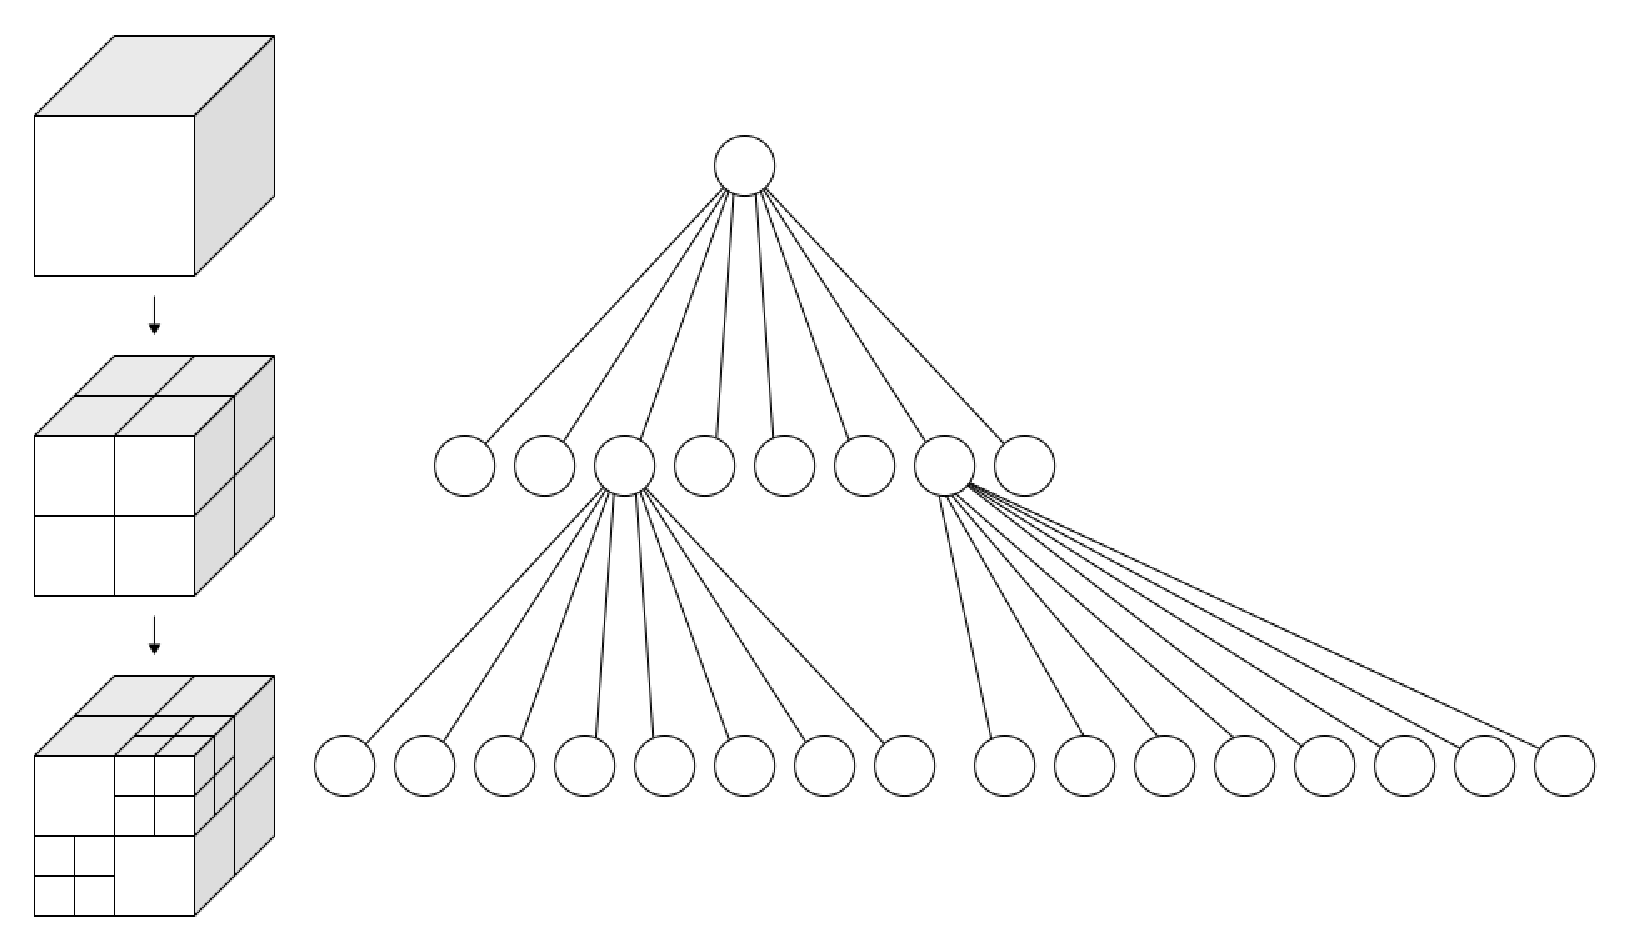
\includegraphics[width=0.8\textwidth]{octree}};
    \end{tikzpicture}
    \caption{Représentation d'un octree}
\end{figure}
\end{frame}
}

\subsection{Complexités}
\begin{frame}
\frametitle{Complexités}
\begin{itemize}
    \itemsep1.5em
    \item Accès : $O(M\frac{\log(N)}{\log(M)})$
    \item Temps de recherche de voisins jusqu'à 10 fois plus rapide pour < 1K
        atomes
    \item Parcours entier à l'arbre
    \item Utilisation de Queue pour le dessin
\end{itemize}
\end{frame}

\section{Agent}

\begin{frame}
\frametitle{Agent}
\usetikzlibrary{arrows.meta}
\tikzset{%
  >={Latex[width=2mm,length=2mm]},
  % Specifications for style of nodes:
            base/.style = {rectangle, rounded corners, draw=black,
                           minimum width=4cm, minimum height=1cm,
                           text centered, font=\sffamily},
  activityStarts/.style = {base, fill=blue!30},
       startstop/.style = {base, fill=red!30},
    activityRuns/.style = {base, fill=green!30},
         process/.style = {base, minimum width=2.5cm, fill=orange!15,
                           font=\ttfamily},
}
\begin{tikzpicture}[node distance=1.5cm,
    every node/.style={fill=white, font=\sffamily}, align=center]

  \node (start)             [Application]              {Application agent starts};
  \node (masterController)     [process, below of=start]          {Controller (MASTER)};
  \node (AtomController)      [process,below of=masterController, right of=ReactionController , xshift=-6cm]   {Atom Controller};
  \node (MolecularController)      [process,below of=masterController, left of=ReactionController, xshift=6 cm]   {Molecule Controller};
  \node (ReactionController)      [process, below of=masterController]   {Reaction Controller};

  \node (atom1)     [process, below of=AtomController]   {Atom ex: H};
  \node (Environment)      [activityRuns, below of=ReactionController]
                                                      {Create Environment};

  \node (atoms)     [activityRuns, yshift=-2cm, below of=Environment]   {Atoms as agents};


  \draw[->]     (start) -- (masterController);
  \draw[->]     (masterController) -- (AtomController);
  \draw[->]     (masterController) --(MolecularController);
  \draw[->]     (masterController) --  (ReactionController);
  \draw[->]     (ReactionController) --  (Environment);
  \draw[->]     (MolecularController) |-  (Environment);
  \draw[->]     (AtomController) --  (atom1);
  \draw[->]     (atom1) |- node[text width=3cm]
                                   {Add atom to environment}  (Environment);
  \draw[->]     (Environment) -- node[text width=3cm]
                                   {contain agents}(atoms);

\end{tikzpicture}
\end{frame}
\section{Aspect moléculaire}

\begin{frame}
\frametitle{Aspect moléculaire}
\begin{itemize}
\item{La formule de Lennard jones }
     \begin{displaymath}
     \phi_{\rm LJ} (r) =  \left[ \left(\frac{A}{r^{12}}\right) - \left(\frac{B}{r^{6}}\right) \right]\end{displaymath}
    
    Oû :
    \begin{itemize}
        \item $ A = 4 \varepsilon \sigma ^{12}$
        \item $ B = 4 \varepsilon \sigma ^{6}$
    \end{itemize}

https://phet.colorado.edu/sims/html/atomic-interactions/latest/atomic-interactions_en.html
\item{L'algorithme de Verlet et les lois de Newton}
\end{itemize}

\end{frame}

\end{document}
